\documentclass[conference]{IEEEtran}
\IEEEoverridecommandlockouts
% The preceding line is only needed to identify funding in the first footnote. If that is unneeded, please comment it out.
\usepackage{cite}
\usepackage{amsmath,amssymb,amsfonts}
\usepackage{algpseudocode}
\usepackage{algorithm}
\usepackage{graphicx}
\usepackage{textcomp}
\usepackage{xcolor}
\usepackage{multirow}
\usepackage{makecell}
\def\BibTeX{{\rm B\kern-.05em{\sc i\kern-.025em b}\kern-.08em
    T\kern-.1667em\lower.7ex\hbox{E}\kern-.125emX}}
\begin{document}

\title{SALCA-IB: Self-Adaptive LLM-Driven Continuous Learning Agent for IB Network Failure Prediction}

%\thanks{Identify applicable funding agency here. If none, delete this.}

%\author{\IEEEauthorblockN{1\textsuperscript{st} Given Name Surname}
%\IEEEauthorblockA{\textit{dept. name of organization (of Aff.)} \\
%\textit{name of organization (of Aff.)}\\
%City, Country \\
%email address or ORCID}
%\and
%\IEEEauthorblockN{2\textsuperscript{nd} Given Name Surname}
%\IEEEauthorblockA{\textit{dept. name of organization (of Aff.)} \\
%\textit{name of organization (of Aff.)}\\
%City, Country \\
%email address or ORCID}
%\and
%\IEEEauthorblockN{3\textsuperscript{rd} Given Name Surname}
%\IEEEauthorblockA{\textit{dept. name of organization (of Aff.)} \\
%\textit{name of organization (of Aff.)}\\
%City, Country \\
%email address or ORCID}
%\and
%\IEEEauthorblockN{4\textsuperscript{th} Given Name Surname}
%\IEEEauthorblockA{\textit{dept. name of organization (of Aff.)} \\
%\textit{name of organization (of Aff.)}\\
%City, Country \\
%email address or ORCID}
%\and
%\IEEEauthorblockN{5\textsuperscript{th} Given Name Surname}
%\IEEEauthorblockA{\textit{dept. name of organization (of Aff.)} \\
%\textit{name of organization (of Aff.)}\\
%City, Country \\
%email address or ORCID}
%\and
%\IEEEauthorblockN{6\textsuperscript{th} Given Name Surname}
%\IEEEauthorblockA{\textit{dept. name of organization (of Aff.)} \\
%\textit{name of organization (of Aff.)}\\
%City, Country \\
%email address or ORCID}
%}

\maketitle

\begin{abstract}
The proliferation of transformer-based large language models has intensified demands on high-performance computing infrastructure, where InfiniBand (IB) networks are crucial for their superior low-latency and high-bandwidth communication capabilities. Network failures in these environments can trigger significant training interruptions or necessitate complete restarts, leading to substantial computational resource waste and training cost overhead. However, effective failure prediction faces dual challenges: the scarcity of failure data and the vulnerability of network features to environmental variations. This paper introduces \textbf{SALCA-IB} (Self-Adaptive LLM-Driven Continuous Learning Agent for IB Network Failure Prediction), an innovative system that leverages Large Language Models (LLMs) as its planning core. The system's key innovations comprise: (1) LLM-driven autonomous data selection and model optimization; (2) A dual-memory fusion system integrating short-term and long-term memory mechanisms; and (3) LLM-supported automatic evaluation feedback with closed-loop optimization. Experimental results on a production cluster with 2,048 computing cards demonstrate that SALCA-IB enhances prediction F1@K-score by 5.1\% in static scenarios and achieves a 19.1\% improvement when confronting network feature distribution shifts, substantially advancing the predictability of large-scale computing infrastructure.
\end{abstract}

\begin{IEEEkeywords}
    InfiniBand Network, Large Language Model, Autonomous Agent
\end{IEEEkeywords}

\section{Introduction}
The unprecedented evolution of transformer-based language models has revolutionized the artificial intelligence landscape, imposing extraordinary demands on computing infrastructure. Training these increasingly sophisticated models, which frequently encompass hundreds of billions of parameters, necessitates extensive distributed computing resources equipped with high-performance interconnects. Within this computational ecosystem, InfiniBand (IB) networks have emerged as the de facto standard, distinguished by their superior low-latency and high-bandwidth communication capabilities, thereby forming the essential backbone for distributed training operations.

Network failures in distributed training environments can have severe consequences. When IB network failures occur during model training, they often trigger unexpected training interruptions or necessitate complete restarts, leading to significant computational resource waste and increased operational costs. For instance, recent studies have shown that network-related failures can account for up to 30\% of training interruptions in large-scale AI clusters, with each incident potentially wasting hundreds of GPU hours (He et al. \cite{b6}). This challenge becomes particularly acute as models grow larger and training runs extend to weeks or even months.

Despite its paramount importance, effective IB network failure prediction confronts multiple fundamental challenges. Primarily, failure data in production environments exhibits inherent scarcity, as failure events remain relatively rare in well-maintained systems, thereby impeding the development of robust prediction models through conventional machine learning approaches. Furthermore, network feature distributions demonstrate high dynamicity and vulnerability to diverse external factors (Liu et al. \cite{b8}), including environmental conditions, hardware degradation, and maintenance interventions. These challenges are intensified by the escalating scale and architectural complexity of modern computing infrastructures.

Traditional approaches to network failure prediction predominantly rely on static machine learning models or rule-based systems (Mohammed et al. \cite{b9}, Nie et al. \cite{b10}). Although these methods demonstrate efficacy in controlled environments, they exhibit significant performance degradation in real-world scenarios where network characteristics undergo continuous evolution. Furthermore, existing solutions typically function as black boxes, offering limited interpretability while failing to effectively utilize historical experience for systematic improvement (Das et al. \cite{b5}). While recent advances in deep learning-based approaches have endeavored to address these limitations, they continue to encounter substantial challenges in adapting to dynamic environments and maintaining sustained prediction accuracy (Alharthi et al. \cite{b2}).

The advent of Large Language Models (LLMs) introduces promising avenues for addressing these challenges. LLMs have exhibited exceptional capabilities in complex reasoning and strategic planning tasks (Ahmed et al. \cite{b1}, Su et al. \cite{b12}), indicating their potential as orchestrators for adaptive prediction systems. Moreover, recent innovations in memory systems and continuous learning architectures (Zhang et al. \cite{b13}) demonstrate significant promise in managing dynamic environments, although their application to IB network failure prediction remains substantially underexplored.

To address these challenges, we propose SALCA-IB (Self-Adaptive LLM-Driven Continuous Learning Agent for IB Network Failure Prediction), an innovative system that combines the reasoning capabilities of LLMs with traditional machine learning models in a unified, adaptive framework. To tackle the data scarcity challenge, SALCA-IB employs an LLM-driven planning core that intelligently orchestrates data selection and model optimization. To handle dynamic feature distributions, we design a dual-memory system that integrates both short-term and long-term experiences. Furthermore, to ensure sustained prediction accuracy, we implement a continuous learning mechanism with LLM-supported feedback loops that enables real-time adaptation to changing network conditions.

The main contributions of this paper are threefold:
\begin{itemize}
    \item We introduce a novel LLM-driven agent architecture for IB network failure prediction that strategically positions LLM as a high-level planning core to orchestrate model selection, parameter optimization, and continuous learning strategies, while deploying traditional machine learning models as efficient executors for real-time prediction tasks.
    \item We develop an innovative dual-memory fusion system that organically integrates short-term and long-term memory mechanisms, facilitating rapid adaptation to dynamic network variations while systematically preserving and leveraging historical knowledge to enhance prediction robustness.
    \item We perform extensive empirical evaluation on a large-scale production cluster comprising 2,048 computing cards, demonstrating that SALCA-IB achieves a 5.1\% improvement in prediction F1@K-score under static conditions and realizes a 19.1\% performance gain when confronting network feature distribution shifts. Through systematic ablation studies, we quantitatively validate the significant contributions of both the LLM-driven framework and the dual-memory system components.
\end{itemize}

The manuscript is structured as follows: Section II examines related work in HPC failure prediction and LLM agent applications. Section III elaborates on the architectural design and implementation details of SALCA-IB. Section IV presents comprehensive experimental methodology and results. Finally, Section V summarizes our findings and outlines future research directions.

\begin{figure*}[htbp]
    \centering
    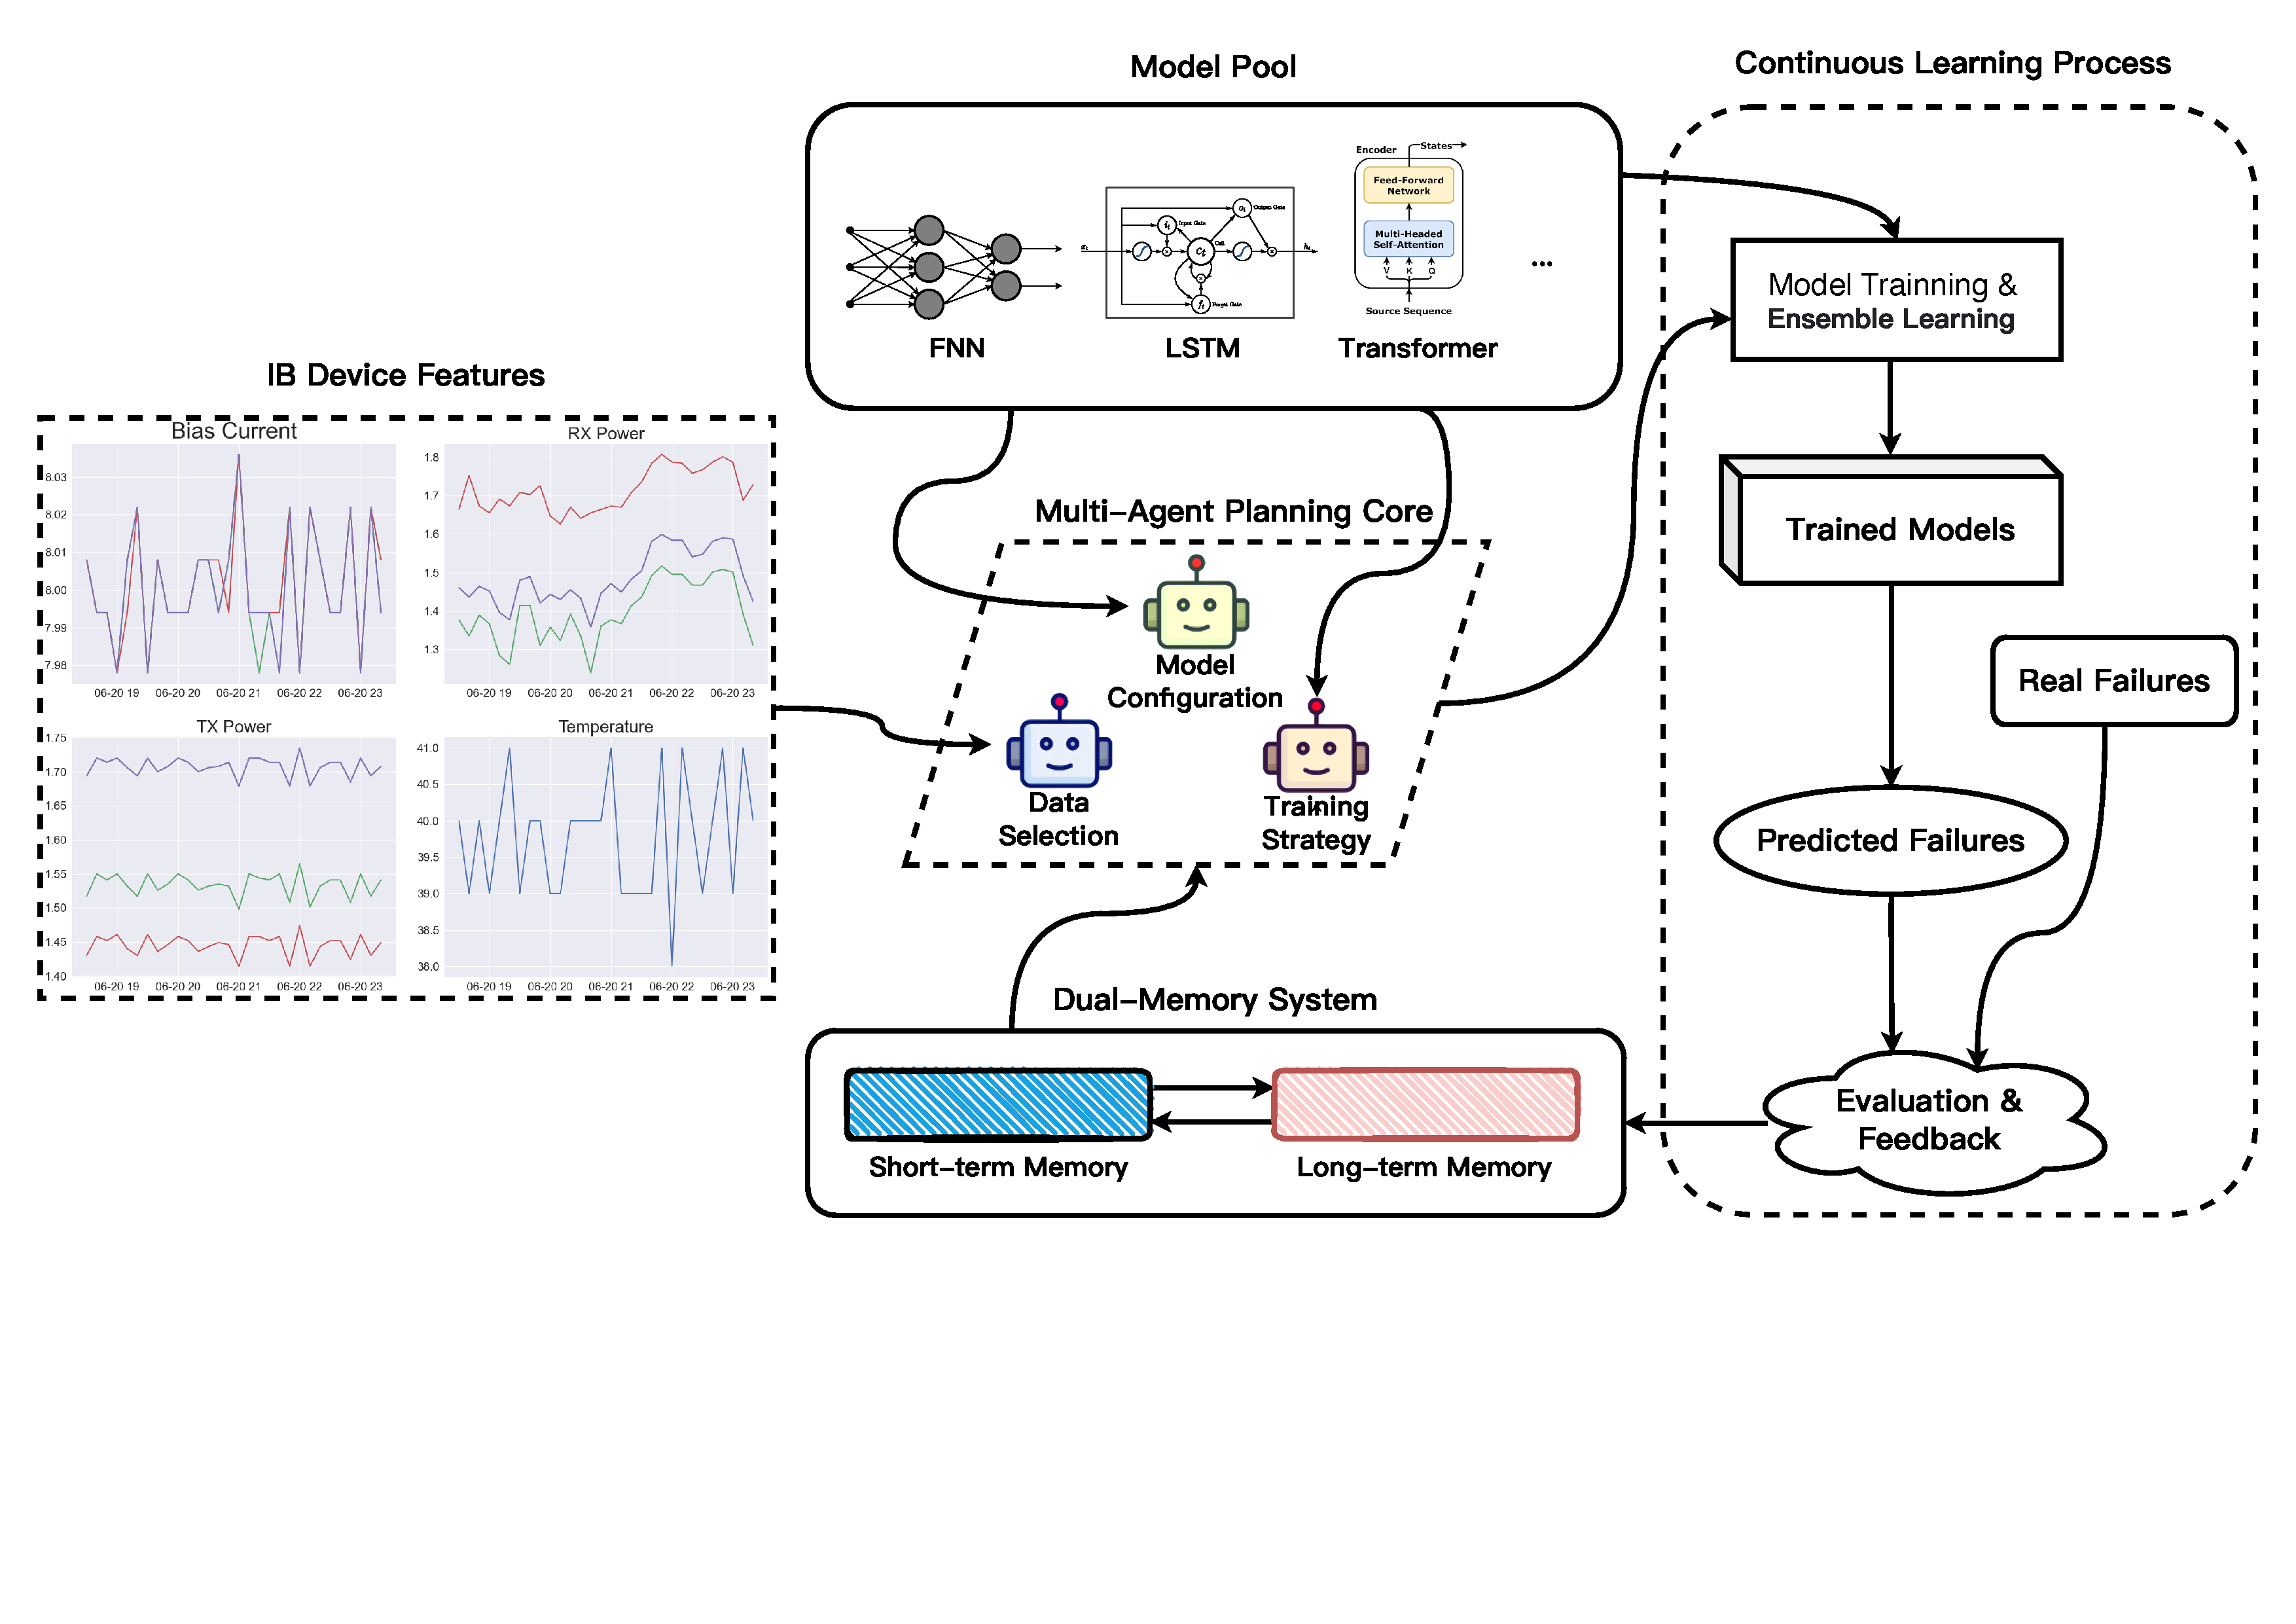
\includegraphics[width=0.95\textwidth]{fig/agent.pdf}
    \caption{Overview of SALCA-IB architecture. The system integrates (a) a model pool containing diverse deep learning models, (b) a multi-agent planning core for intelligent orchestration, (c) a dual-memory system for knowledge retention, and (d) a continuous learning process for adaptive optimization.}
    \label{fig:salca-ib}
\end{figure*}


\section{Related Work}

\subsection{HPC Clusters Failure Prediction}
Failure prediction in HPC clusters, particularly for large-scale GPU training workloads, has garnered substantial research attention due to its fundamental role in maintaining system reliability. Conventional methodologies predominantly employ statistical analysis and machine learning techniques. He et al. \cite{b6} conducted comprehensive analyses of hardware failures in deep learning training systems, establishing that GPU failures substantially impact training progression and model convergence. In parallel, Liu et al. \cite{b8} specifically investigated GPU failure prediction under intensive deep learning workloads, illuminating the distinctive challenges inherent in monitoring and predicting failures within GPU-intensive computing environments.

Contemporary research has endeavored to address these challenges through ensemble methodologies and advanced deep learning approaches. Nie et al. \cite{b10} pioneered GPU error prediction models leveraging temporal and spatial dependencies to enhance prediction robustness under data-constrained conditions, conceptually aligned with our model pool architecture albeit lacking intelligent orchestration capabilities. Das et al. \cite{b5} investigated LSTM-based architectures for system health prediction and failure lead time estimation, sharing conceptual similarities with our long-term memory mechanism but without incorporating continuous adaptation mechanisms. Liu et al. \cite{b8} further advanced the field through high-precision GPU failure prediction methods under deep learning workloads, demonstrating enhanced accuracy while still encountering limitations in dynamic environments. Despite these advancements, as emphasized by Alharthi et al. \cite{b2}, existing methodologies continue to face substantial challenges in managing dynamic network environments and maintaining sustained prediction accuracy.

\subsection{LLM-based Reasoning and Self-Improvement}
Recent advancements in LLM capabilities have revealed their significant potential in complex reasoning and self-improvement tasks. This evolution can be examined through two distinct perspectives:

\subsubsection{Reasoning and Verification}
LLMs have exhibited exceptional capabilities in complex reasoning tasks, albeit with specific constraints that warrant careful consideration. Chen et al. \cite{chen2023} established chain-of-thought prompting as a fundamental methodology for enhancing reasoning capabilities, while Wang et al. \cite{wang2023} extended this paradigm through a self-consistency framework that systematically evaluates multiple reasoning pathways. An et al. \cite{an2024} subsequently demonstrated LLMs' capacity to enhance reasoning capabilities through error-driven learning, particularly when provided with structured feedback mechanisms. However, Tyen et al. \cite{tyen2023} identified a critical limitation: while LLMs excel at guided correction, they exhibit significant limitations in autonomous error detection.

Contemporary research has focused on addressing these inherent limitations through diverse methodological approaches. Weng et al. \cite{weng2023} developed sophisticated self-verification mechanisms that substantially enhance reasoning reliability. Complementarily, Gou et al. \cite{gou2024} introduced CRITIC, an innovative framework enabling LLMs to perform self-correction through tool-interactive critiquing. These advancements in self-improvement capabilities hold particular significance for complex system monitoring and failure prediction tasks, where precise reasoning about system states is paramount.

\subsubsection{Continuous Learning and Adaptation}
The evolution of continuous learning capabilities in LLMs has demonstrated remarkable progress, particularly regarding their capacity for temporal adaptation and improvement. Madaan et al. \cite{madaan2023} pioneered a self-improving framework wherein LLMs autonomously generate and evaluate optimization strategies. This foundational work was further enhanced by Gao et al. \cite{gao2024}, who developed a comprehensive lifelong learning approach facilitating autonomous experiential learning in LLMs.

Several innovative frameworks have emerged to augment LLMs' adaptive capabilities. Qiao et al. \cite{qiao2024} demonstrated enhanced tool learning through systematic execution feedback, while Shinn et al. \cite{shinn2023} introduced Reflexion, a sophisticated framework for implementing verbal reinforcement learning in language agents. These advances in continuous learning and adaptation mechanisms prove particularly pertinent for maintaining prediction accuracy in dynamic operational environments.

\subsection{LLM Applications in Time Series and Agent Systems}
The integration of LLMs into time series analysis and agent-based systems represents an emerging research frontier, with particular relevance to failure prediction tasks.

\subsubsection{Time Series Analysis and Forecasting}
Recent investigations have demonstrated LLMs' efficacy in time series analysis tasks. Gruver et al. \cite{gruver2023} established the feasibility of zero-shot time series forecasting using LLMs, while Jin et al. \cite{jin2024} developed Time-LLM, illustrating the potential for reprogramming LLMs specifically for time series forecasting applications. Cao et al. \cite{cao2024} introduced TEMPO, a sophisticated prompt-based framework engineered for precise time series prediction.

Contemporary methodological advances have focused on enhancing LLMs' temporal data processing capabilities. Chang et al. \cite{chang2024} developed novel techniques for optimizing pre-trained LLMs as data-efficient time series forecasters, while Zhou et al. \cite{zhou2023} established a unified paradigm for comprehensive time series analysis utilizing pretrained language models. Xue et al. \cite{xue2023} introduced PromptCast, pioneering an innovative prompt-based learning framework specifically engineered for time series forecasting tasks.

\subsubsection{Multi-Agent and Workflow Systems}
The incorporation of LLMs into multi-agent and workflow systems has emerged as a promising paradigm for complex task orchestration. Wang et al. \cite{wang2024} demonstrated that mixture-of-agents architectures substantially enhance LLM capabilities, particularly in managing complex, multi-step operational sequences. Wang et al. \cite{wang2024agent} pioneered agent workflow memory systems, addressing fundamental challenges in maintaining state consistency across extended operations.

These architectural advances have demonstrated particular efficacy in domain-specific applications. Yao et al. \cite{yao2023} established the viability of LLM-based approaches for multi-agent reasoning and action coordination, illustrating their potential for orchestrating complex, multi-entity prediction tasks. While these developments represent significant progress in both LLM capabilities and their practical applications, their potential for network failure prediction remains substantially underexplored, particularly regarding the challenges of dynamic network environments and real-time adaptation requirements.

\section{Methodology}

SALCA-IB is designed as a self-adaptive intelligent system that leverages large language models (LLMs) to orchestrate network failure prediction in industrial blockchain environments. As illustrated in Fig. \ref{fig:salca-ib}, the system integrates four key components: an LLM-driven planning core, a dual-memory system, a deep learning model pool, and a continuous learning process.

As shown in Algorithm \ref{alg:salca-ib}, the LLM planning core serves as the system's central intelligence, orchestrating model selection, data processing, and strategy optimization. The dual-memory system combines short-term memory for rapid response and long-term memory for knowledge retention, enabling both immediate adaptation and sustained optimization. The model pool comprises diverse deep learning models (MLP, LSTM, and Transformer) that serve as the execution layer for failure prediction. Through continuous learning, the system evaluates prediction outcomes and adjusts strategies dynamically, ensuring robust performance in evolving network conditions. The detailed design of each component is elaborated in the following sections.

\subsection{LLM-Driven Planning Core}
Traditional failure prediction systems often rely on static model architectures and fixed training strategies, limiting their effectiveness in dynamic IB environments. Our LLM-driven planning core addresses this challenge by orchestrating three key components: data selection, model configuration, and training strategy optimization, as shown in Fig. \ref{fig:salca-ib}.

\subsubsection{Data Selection}
The data selection module processes IB network data streams $\mathcal{D} = \{(X_t, y_t)\}_{t=1}^T$, where $X_t \in \mathbb{R}^{w \times d}$ represents a sequence of network states within a sliding window. Specifically, $X_t = [x_{t-w+1}, ..., x_t]$ where $x_i \in \mathbb{R}^d$ contains $d$ network features at time step $i$, $w$ is the window size (e.g., 30 time steps), and $y_t \in \{0,1\}$ indicates whether a failure occurs following this sequence. Given historical knowledge $\mathcal{K} \subset Mem_{long}$, the LLM performs reasoning-based selection through:

\begin{equation}
    \mathcal{D}_{train} = f_{LLM}(\mathcal{D}, \mathcal{K}) = \{(X_i, y_i) | s_i > \tau, (X_i, y_i) \in \mathcal{D}\}
\end{equation}

where $s_i$ is the sequence importance score determined by LLM reasoning:
\begin{equation}
    s_i = LLM(X_i, \mathcal{K}, \text{prompt}_{select})
\end{equation}

The LLM generates importance scores through a structured reasoning process that evaluates both temporal evolution patterns and feature interactions within each sequence. This evaluation process is guided by carefully designed prompts that encode domain knowledge about network failure progression patterns and their manifestation across multiple features over time.

The data selection process consists of three sequential components:

\textit{a) Temporal Window Selection}: The LLM analyzes temporal context to determine optimal window configuration:
\begin{equation}
    W_t^* = LLM(\{X_{t-k}, ..., X_t\}, \mathcal{K}, \text{prompt}_{temporal})
\end{equation}
where $\text{prompt}_{temporal}$ guides the analysis of multi-scale temporal dependencies. The window selection considers both the granularity of individual time steps and the overall sequence length needed to capture failure progression patterns.

\textit{b) Distribution Assessment}: For selected windows, the LLM evaluates sequence representativeness:
\begin{equation}
    q_i = LLM(X_i, W_t^*, \mathcal{K}, \text{prompt}_{distribution})
\end{equation}
This assessment examines both the temporal evolution of individual features and their cross-feature correlations within each sequence. The evaluation particularly focuses on identifying characteristic patterns that historically preceded failure events.

\textit{c) Final Selection}: The LLM integrates previous analyses for final sequence selection:
\begin{equation}
    \mathcal{D}_{train} = \{(X_i, y_i) | LLM(q_i, \mathcal{K}, \text{prompt}_{final}) > \tau\}
\end{equation}
The final selection phase considers the completeness and quality of feature sequences, ensuring selected samples contain meaningful progression patterns for failure prediction.

The prompt design for each component incorporates specific aspects of temporal sequence analysis and feature interaction patterns. This enables the LLM to identify and select sequences that best capture the progression of network states leading to potential failures, while considering both historical patterns and current network conditions.

\subsubsection{Model Configuration}
The model configuration module dynamically selects and configures prediction models based on both current data characteristics and historical performance patterns. Given a model pool $\mathcal{M} = \{M_1, ..., M_m\}$ containing various neural architectures (e.g.,CNN, LSTM, Transformer), the LLM performs configuration through:

\begin{equation}
    (M_{selected}, \Theta, S) = f_{LLM}^{config}(\mathcal{M}, \mathcal{K}, X_t)
\end{equation}

where $M_{selected} \subset \mathcal{M}$ is the selected model subset, $\Theta$ represents their corresponding parameter configurations, and $S$ defines the ensemble strategy. The configuration process consists of three key components:

\textit{a) Architecture Selection}: The LLM evaluates and selects appropriate model architectures based on current sequence characteristics:
\begin{equation}
    M_{selected} = LLM(\mathcal{M}, X_t, \mathcal{K}, \text{prompt}_{arch})
\end{equation}
This selection considers the temporal dependency patterns in $X_t$, such as choosing LSTM for strong short-term dependencies or Transformer for capturing long-range correlations. The historical performance records in $\mathcal{K}$ guide this selection by providing evidence of each architecture's effectiveness under similar conditions.

\textit{b) Parameter Configuration}: For each selected model $M_i \in M_{selected}$, the LLM determines its optimal configuration:
\begin{equation}
    \theta_i = LLM(M_i, X_t, \mathcal{K}, \text{prompt}_{param})
\end{equation}
where $\theta_i \in \Theta$ includes both architectural parameters (e.g., number of layers, hidden dimensions) and training parameters (e.g., learning rate, batch size). The configuration is based on both the current data characteristics and historical configuration effectiveness stored in $\mathcal{K}$.

\textit{c) Ensemble Strategy Design}: The LLM designs an ensemble strategy $S$ that optimally combines the selected models:
\begin{equation}
    S = LLM(M_{selected}, \Theta, \mathcal{K}, \text{prompt}_{ensemble})
\end{equation}
The ensemble strategy includes both the voting mechanism and individual model weights, determined by analyzing each model's historical reliability and current data fitness. The final ensemble model is constructed as:
\begin{equation}
    M_{ensemble}(X_t) = \sum_{i=1}^{|M_{selected}|} w_i M_i(X_t; \theta_i)
\end{equation}
where $w_i$ represents the dynamic weight assigned to each model's prediction.

This knowledge-driven configuration process enables the system to adapt its prediction models dynamically based on evolving network conditions while leveraging accumulated experience from historical operations.

\subsubsection{Training Strategy}
The training strategy module optimizes the learning process of the ensemble model through LLM-driven adaptation. Given the selected training data $\mathcal{D}_{train}$ and configured ensemble model $M_{ensemble}$, the training process is formulated as:

\begin{equation}
    M_{ensemble}^* = f_{LLM}^{train}(M_{ensemble}, \mathcal{D}_{train}, \mathcal{K})
\end{equation}

The training optimization process consists of three key components:

\textit{a) Initial Parameter Configuration}: For each model $M_i$ in the ensemble, the LLM determines optimal training parameters based on historical experience:
\begin{equation}
    \{\eta_i, B_i\} = LLM(M_i, \mathcal{D}_{train}, \mathcal{K}, \text{prompt}_{init})
\end{equation}
where $\eta_i$ is the fixed learning rate and $B_i$ is the batch size for model $M_i$. These parameters remain constant throughout the training process, with their values determined by analyzing historical training patterns stored in $\mathcal{K}$.

\textit{b) Loss Function Design}: The LLM constructs a composite loss function based on prediction requirements and historical error patterns:
\begin{equation}
    \begin{aligned} 
    \mathcal{L}(X_t, y_t) = \alpha\mathcal{L}_{ce}(X_t, y_t) &+ \beta\mathcal{L}_{temporal}(X_t) \\
    &+ \gamma\mathcal{L}_{reg}(M_{ensemble})
    \end{aligned}
\end{equation}
where $\mathcal{L}_{ce}$ is the cross-entropy loss for failure prediction, $\mathcal{L}_{temporal}$ penalizes temporal inconsistency in predictions, and $\mathcal{L}_{reg}$ provides regularization based on historical failure patterns. The weights $\alpha, \beta, \gamma$ are determined before training:
\begin{equation}
    [\alpha, \beta, \gamma] = LLM(\mathcal{D}_{train}, \mathcal{K}, \text{prompt}_{loss})
\end{equation}

\textit{c) Performance Monitoring}: The LLM continuously evaluates prediction performance and triggers model updates when necessary:
\begin{equation}
    \delta_t = LLM(M_{ensemble}, X_t, \mathcal{K}, \text{prompt}_{monitor})
\end{equation}
where $\delta_t$ is the update decision signal. When significant performance degradation is detected, the system initiates retraining with newly configured parameters:
\begin{equation}
    M_{ensemble}^{t+1} = \begin{cases}
        \text{Retrain}(M_{ensemble}, \mathcal{D}_{new}, \{\eta_i^{new}\}) & \text{if } \delta_t > \tau \\
        M_{ensemble}^t & \text{otherwise}
    \end{cases}
\end{equation}

This framework ensures stable training processes while maintaining the flexibility to adapt to significant changes in network conditions through model retraining with newly optimized parameters.

\subsection{Dual-Memory System}
The dual-memory system implements a JSON-based knowledge repository that facilitates efficient experience accumulation and retrieval for LLM-driven decision making. This system addresses the context length limitations of LLMs while enabling continuous learning through structured knowledge preservation.

\subsubsection{Memory Architecture}
The short-term memory maintains a dynamic operational context for immediate decision support:
\begin{equation}
    Mem_{short} = \{F_{current}, T_{range}, P_{model}, M_{config}, F_{recent}\}
\end{equation}
where $F_{current}$ represents the active feature set with selection rationale, $T_{range}$ captures temporal context with start and end timestamps, $P_{model}$ stores recent model performance metrics, and $M_{config}$ maintains current model configurations and ensemble strategies.

The long-term memory implements a persistent knowledge base with activation tracking:
\begin{equation}
    Mem_{long} = \{F_{stats}, M_{history}, E_{record}, A_{track}, F_{history}\}
\end{equation}
where $F_{stats}$ maintains feature statistics and selection history, $M_{history}$ records successful model configurations, $E_{record}$ stores historical experience entries, $A_{track}$ tracks memory activation patterns, and $F_{history}$ maintains valuable historical feedback:
\begin{equation}
    F_{history} = \{(f_i, t_i, e_i) | Q(f_i) > \tau_{feedback}\}
\end{equation}

Each feedback entry contains:
\begin{equation}
    f_i = \{P_i, R_i, A_i\}
\end{equation}
where $P_i$ represents performance metrics, $R_i$ captures LLM reasoning, and $A_i$ records adaptation decisions.

\subsubsection{Memory Operations}
The system implements three basic memory operations:

\textit{a) Experience Recording}: The system records new operational experiences in short-term memory:
\begin{equation}
    Mem_{short}^{t+1} = Record(X_t, y_t, P_t, C_t)
\end{equation}
where $X_t$ represents current feature data, $y_t$ is the prediction outcome, $P_t$ contains performance metrics, and $C_t$ includes current configurations.

\textit{b) Memory Transfer}: The system periodically transfers valuable experiences from short-term to long-term memory:
\begin{equation}
    Mem_{long}^{t+1} = Transfer(Mem_{short}, Mem_{long})
\end{equation}
This operation includes recording successful feature selections, model configurations, and performance patterns.

\textit{c) Activation-based Cleanup}: The system implements an activation-aware cleanup mechanism:
\begin{equation}
    A_{score}(e_i) = \lambda\frac{t_{current} - t_{last}(e_i)}{T_{max}} + (1-\lambda)\frac{n_{access}(e_i)}{N_{max}}
\end{equation}
where $\lambda$ balances recency and frequency of access. The cleanup operation removes entries based on their activation scores:
\begin{equation}
    Mem_{clean} = \{e_i | A_{score}(e_i) > \tau_{active}\}
\end{equation}
where $\tau_{active}$ is the retention threshold.

The system maintains its effectiveness through activation-aware memory management, ensuring both efficiency and relevance in supporting LLM-driven decisions.
    
\subsection{Continuous Learning Process}
The continuous learning process implements a self-evolving mechanism through LLM-driven optimization and structured feedback analysis. This process establishes a closed-loop learning cycle that continuously refines prediction capabilities based on operational experiences.

\subsubsection{Performance-Driven Feedback Generation}
The system generates structured feedback based on actual prediction results:
\begin{equation}
    P_t = \{accuracy_t, precision_t, recall_t, stability_t\}
\end{equation}
where performance metrics are analyzed through LLM reasoning to generate comprehensive feedback:
\begin{equation}
    f_t = LLM(P_t, E_{record}, \text{prompt}_{analyze})
\end{equation}
The feedback contains component-wise assessments:
\begin{equation}
    f_t = \{(c_i, s_i, r_i) | c_i \in \{feature, model, training\}\}
\end{equation}
where $s_i$ indicates performance status and $r_i$ provides specific improvement recommendations.

\subsubsection{Actionable Improvement Strategy}
Based on the feedback analysis, the system generates concrete improvement strategies:
\begin{equation}
    I_t = LLM(f_t, F_{history}, \text{prompt}_{improve})
\end{equation}
where $I_t$ specifies actionable adjustments:
\begin{equation}
    I_t = \{(a_i, p_i, \Delta_i) | a_i \in Actions\}
\end{equation}
Here, $a_i$ represents specific actions, $p_i$ indicates their priority, and $\Delta_i$ defines the adjustment magnitude.

\subsubsection{Self-Refinement Process}
The system implements a three-stage refinement process:

\textit{a) Strategy Validation}: Proposed improvements are validated against historical experiences:
\begin{equation}
    V_t = LLM(I_t, F_{history}, \text{prompt}_{validate})
\end{equation}

\textit{b) Component Optimization}: Validated strategies are applied to system components:
\begin{equation}
    C_{t+1} = Optimize(C_t, V_t, \text{prompt}_{refine})
\end{equation}
where $C_t$ represents the current configuration of features, models, or training parameters.

\textit{c) Effectiveness Assessment}: The system evaluates optimization outcomes:
\begin{equation}
    E_t = Assess(C_{t+1}, P_{t+1}, \text{prompt}_{assess})
\end{equation}

The assessment results are integrated into the feedback history to guide future improvements:
\begin{equation}
    F_{history}^{t+1} = Update(F_{history}, E_t, \text{prompt}_{update})
\end{equation}

This closed-loop self-refining process and its integration with the dual-memory system ensures continuous improvement while maintaining operational efficiency through experience-based optimization.

The overall framework is summarized in Algorithm \ref{alg:salca-ib}.



\section{Experimental Evaluation}

\begin{table*}[!t]
\caption{Performance Comparison of Different Methods on IB Network Failure Prediction}
\label{tab:main_results}
\renewcommand{\arraystretch}{1.2}
\centering
\begin{tabular}{l|ccc|ccc}
\hline\hline
\multirow{2}{*}{\textbf{Method}} & \multicolumn{3}{c|}{\textbf{Static Scenario}} & \multicolumn{3}{c}{\textbf{Dynamic Scenario}} \\
\cline{2-7}
& P@K (\%) & R@K (\%) & F1@K (\%) & P@K (\%) & R@K (\%) & F1@K (\%) \\
\hline
\multicolumn{7}{l}{\textit{Individual Models}} \\
\hline
MLP & 71.2±1.8 & 67.5±2.1 & 69.3±2.0 & 56.4±3.2 & 52.8±3.5 & 54.5±3.4 \\
CNN & 75.8±1.5 & 71.9±1.8 & 73.8±1.7 & 59.8±2.9 & 56.2±3.2 & 57.9±3.1 \\
LSTM & 77.2±1.3 & 73.4±1.6 & 75.2±1.5 & 63.5±2.6 & 59.9±2.9 & 61.6±2.8 \\
GRU & 78.1±1.2 & 74.2±1.5 & 76.1±1.4 & 64.8±2.5 & 61.2±2.8 & 62.9±2.7 \\
Transformer & 80.3±1.1 & 76.5±1.4 & 78.3±1.3 & 67.2±2.4 & 63.6±2.7 & 65.3±2.6 \\
\hline
\multicolumn{7}{l}{\textit{Traditional Ensemble Methods}} \\
\hline
Majority Voting & 81.5±1.0 & 77.8±1.2 & 79.6±1.1 & 63.8±2.2 & 60.2±2.5 & 61.9±2.4 \\
Weighted Voting & 82.4±0.9 & 78.6±1.1 & 80.4±1.0 & 65.9±2.1 & 62.3±2.4 & 64.0±2.3 \\
\hline
\multicolumn{7}{l}{\textit{LLM-based Methods (with GPT-4o)}} \\
\hline
End-to-End Prompting & 67.2±1.8 & 63.5±2.0 & 65.3±1.9 & 63.9±2.4 & 60.4±2.7 & 62.1±2.6 \\
Chain-of-Thought & 68.5±1.7 & 64.8±1.9 & 66.6±1.8 & 65.7±2.3 & 62.2±2.6 & 63.9±2.5 \\
Self-Refine & 69.1±1.6 & 65.4±1.8 & 67.2±1.7 & 67.3±2.2 & 63.8±2.5 & 65.5±2.4 \\
\hline
\multicolumn{7}{l}{\textit{SALCA-IB with Different LLM Cores}} \\
\hline
SALCA-IB (Qwen2.5-14B) & 77.8±1.3 & 74.1±1.5 & 75.9±1.4 & 70.2±2.2 & 67.1±2.5 & 68.6±2.4 \\
SALCA-IB (Yi-1.5-34B) & 83.2±0.9 & 79.5±1.1 & 81.3±1.0 & 77.5±1.8 & 74.2±2.1 & 75.8±2.0 \\
SALCA-IB (Llama-3-70B) & 84.5±0.8 & 80.8±1.0 & 82.6±0.9 & 79.6±1.7 & 76.5±2.0 & 78.0±1.9 \\
\textbf{SALCA-IB (GPT-4o)} & \textbf{87.2±0.7} & \textbf{83.9±0.9} & \textbf{85.5±0.8} & \textbf{84.7±1.6} & \textbf{81.6±1.9} & \textbf{83.1±1.8} \\

\hline\hline
\end{tabular}
\end{table*}

\subsection{Dataset Construction and Collection}

\subsubsection{Infrastructure Overview}
Our experimental environment consists of a large-scale InfiniBand cluster designed for high-performance computing workloads, particularly focused on training large language models exceeding 200 billion parameters. Such training tasks demand exceptional network performance and reliability, as network failures can significantly impact model convergence and training efficiency. The cluster implements a two-layer Leaf-Spine topology with full-mesh connectivity, comprising 2,048 computing cards distributed across 8 pods. Each pod contains 256 cards connected through 8 LEAF switches, with the overall network infrastructure including 64 Leaf switches and 32 Spine switches. This architecture, compliant with NVIDIA's rail-optimized specifications, ensures optimal bandwidth utilization and minimal communication latency while maintaining network redundancy, which is crucial for sustaining the massive data transfers required in distributed LLM training.

Through our analysis, we identified two primary categories of network failures in this infrastructure: link flapping and complete link down events. These failures are particularly critical in LLM training scenarios, where even brief network interruptions can lead to significant training delays or potential loss of computation resources. The failures typically originate from optical module degradation under sustained exposure to adverse environmental conditions, particularly in scenarios involving high-temperature operation and sustained high workloads characteristic of intensive LLM training operations. 

\subsubsection{Data Collection}
We developed a comprehensive data collection framework that integrates four complementary monitoring approaches. System performance counters provide detailed insights into network interface card (NIC) performance and local link status. The OpenSM subnet manager logs capture network-wide connectivity status and state transitions across all devices. Hardware diagnostics data collected through management interfaces provides information about physical components including NICs, optical modules, and cables. Additionally, network topology information is gathered to maintain a complete map of physical connections between devices. 

The final processed dataset demonstrates significant scale and comprehensiveness. The performance metrics data includes approximately 77.8 billion data points collected over eight months, comprising 55 metrics per InfiniBand card (36 performance and error diagnostic metrics, 2 temperature indicators, and 17 physical parameters) collected from 256 nodes, each equipped with 8 IB cards, sampled twice per minute. Real-time state snapshots contribute an additional 40 million records, capturing every network state change. The OpenSM subnet manager logs contain 20.18 million entries documenting network events and state transitions. 

For the failure prediction task, we employ a similar sampling strategy with Liu et al. \cite{b8} for training and evaluation phases. During training, we maintain a balanced 1:1 ratio between failure and normal samples to ensure the model learns effectively from both classes. For evaluation and real-world prediction scenarios, we use a more realistic 1:8 ratio that better reflects the natural distribution of failure events in production environments. 


\subsection{Experimental Setup}

\subsubsection{Implementation Details}
To investigate how LLM reasoning capabilities affect the performance of our SALCA-IB framework, we conducted experiments with four different large language models: GPT-4o (accessed via OpenAI's API), Llama-3-70B-Instruct, Yi-1.5-34B-Chat, and Qwen2.5-14B-Instruct. Each experiment uses a single LLM as the reasoning engine throughout the entire process, allowing us to evaluate how models of different sizes and reasoning capabilities impact the framework's effectiveness. The locally deployed models (Llama-3, Yi-1.5, and Qwen2.5) run on Nvidia H100 GPUs using vLLM for optimized inference.

The prediction model pool consists of lightweight neural networks optimized for CPU inference. These models were trained on our IB network dataset using CPU resources to ensure efficient deployment in production environments. Table \ref{tab:model_config} shows the configuration search space and LLM selection examples.

\subsubsection{Baseline Methods}
We designed three categories of baseline methods to evaluate the effectiveness of our SALCA-IB framework:

\textbf{Individual Deep Learning Models:} We first evaluated each model from our model pool independently. The MLP model serves as a basic deep learning baseline with its hierarchical feature extraction capability. The LSTM and GRU models represent sequence modeling approaches that capture temporal dependencies in network states. The Transformer model provides a self-attention based baseline that can model long-range dependencies. The CNN model is included to capture spatial hierarchies and local patterns in the data, which can be particularly useful for identifying localized anomalies. Each model was trained with its optimal configuration as determined by grid search.

\textbf{Traditional Ensemble Methods:} We then combined these deep learning models using conventional ensemble strategies:
(1) Majority Voting, where each model contributes equally to the final prediction;
(2) Weighted Voting, where weights are assigned based on each model's validation performance;
These ensemble methods represent traditional approaches to model combination without dynamic adaptation.

\textbf{LLM-based Methods:} To isolate the contribution of LLM orchestration, we implemented several LLM-based approaches using the same set of base models. These include End-to-End prompting, Chain-of-Thought prompting \cite{chen2023}, and Self-Refine \cite{madaan2023}. For consistency and fair comparison, each method was tested using the GPT-4o API, aligning with SALCA-IB's LLM-driven orchestration mechanism.

\subsection{Evaluation Methodology}

\subsubsection{Evaluation Scenarios}
The experimental evaluation, conducted on our 8-month dataset, encompasses two distinct scenarios to comprehensively assess system performance. The static scenario evaluates models within a fixed 2-week time window, utilizing 70\% of the data for training and 30\% for testing, enabling assessment of baseline prediction accuracy under stable network conditions.

For dynamic scenario evaluation, we selected a continuous 16-week period from the dataset, where significant maintenance events naturally occurred. The system was initially trained on the first 2-week data segment, followed by continuous evaluation over the subsequent 14 weeks. Two major maintenance events were recorded during this period: a Week 6 maintenance involving optical module replacements and firmware updates, and a Week 12 maintenance encompassing topology adjustments and switch configuration optimization. These events created natural feature distribution shifts, allowing evaluation of the system's adaptability to environmental changes.

\subsubsection{Evaluation Metrics}
The performance assessment employs ranking-based metrics with K set to 2\% of total instances. Precision@K measures the proportion of true positives among predicted positives in top-K predictions. Recall@K quantifies the ratio of detected true positives to actual positives within top-K predictions. F1@K represents the harmonic mean of Precision@K and Recall@K, providing a balanced measure of prediction performance.

Statistical robustness is ensured through five independent experimental runs with different random seeds. Results are presented as mean values with standard deviations, and statistical significance is validated using paired t-tests (p < 0.05). The system is evaluated on its ability to provide failure predictions within a 30-minute advance warning window, a critical requirement for practical deployment in production environments.


\subsection{Main Results}
Table \ref{tab:main_results} presents a comprehensive comparison of SALCA-IB against various baseline approaches. In static scenarios, SALCA-IB with GPT-4o achieves an F1@K score of 85.5±0.8\%, significantly outperforming both traditional machine learning methods and existing LLM-based approaches. Specifically, it surpasses the best performing baseline (Weighted Voting: 80.4±1.0\%) by 5.1\%, and demonstrates substantial improvements over individual models (Transformer: 78.3±1.3\%). The LLM-driven autonomous data selection and model optimization mechanism proves particularly effective, as evidenced by the consistent performance improvements across different model scales (14B: 75.9\%, 34B: 81.3\%, 70B: 82.6\%, GPT-4o: 85.5\%). Notably, the significant performance jump between 14B and 34B models (5.4\% increase) suggests that effective data selection and model optimization require sophisticated reasoning capabilities that only larger LLMs can provide. This observation aligns with our findings that direct LLM-based prediction methods show limited performance (Self-Refine: 67.2±1.7\%) compared to traditional approaches, validating our architectural choice of utilizing LLMs as planning cores rather than predictors.

The advantages of SALCA-IB become even more pronounced in dynamic scenarios where network feature distributions shift. While traditional methods experience severe performance degradation (Transformer: -16.6\%, Weighted Voting: -16.4\%), SALCA-IB (GPT-4o) maintains remarkably stable performance with an F1@K score of 83.1±1.8\%, representing only a 2.4\% decrease from its static scenario performance. Interestingly, basic LLM-based methods demonstrate better resilience to distribution shifts (Self-Refine: -2.5\%, CoT: -4.1\%) compared to traditional models, though their absolute performance remains lower. This observation reinforces the value of incorporating LLM capabilities into our system design. The effectiveness of our dual-memory approach is consistently observed across different LLM scales, with even the 34B variant (75.8±2.0\%) significantly outperforming all baseline methods.

The system's resilience is further enhanced by our automatic evaluation feedback and closed-loop optimization mechanism, as reflected in the performance stability across different scenarios. This is evidenced by the smaller standard deviations in SALCA-IB (GPT-4o) results (±0.8\% static, ±1.8\% dynamic) compared to traditional approaches (±1.0-2.6\%). The contrast between SALCA-IB's resilience and the performance variations in traditional approaches demonstrates that our system successfully maintains high performance levels through continuous adaptation and optimization, while effectively leveraging the inherent adaptability of LLMs in dynamic environments.

\begin{table}[!t]
\caption{Ablation Study Results}
\label{tab:ablation}
\renewcommand{\arraystretch}{1.2}
\begin{center}
\begin{tabular}{l|cc}
\hline\hline
\textbf{Model Variant} & \textbf{Static} & \textbf{Dynamic} \\
& \textbf{F1@K (\%)} & \textbf{F1@K (\%)} \\
\hline
SALCA-IB (Full) & \textbf{85.5±0.8} & \textbf{83.1±1.8} \\
\hline
w/o LLM Planning & 79.8±1.3 & 67.2±2.4 \\
w/o Dual Memory & 81.3±1.2 & 73.5±2.2 \\
w/o Continuous Learning & 82.9±1.0 & 76.8±2.0 \\
\hline
Weighted Voting & 80.4±1.0 & 64.0±2.3 \\
\hline\hline
\end{tabular}
\end{center}
\end{table}

\subsection{Ablation Studies}
To validate the effectiveness of each key component in SALCA-IB, we conducted ablation experiments by removing individual components while keeping others intact. Table \ref{tab:ablation} presents the performance comparison between the full system and its variants, alongside the weighted voting baseline.

The LLM planning core demonstrates its effectiveness through the significant performance gap between the full system and the variant without LLM planning. In static scenarios, the absence of LLM planning leads to a 5.7\% decrease in F1@K score, while in dynamic scenarios, the impact is even more pronounced with a 15.9\% decrease. Without the LLM planning core, SALCA-IB essentially degrades into a traditional ensemble learning system with rule-based model selection and fixed data sampling strategies. The performance (79.8\% in static scenarios and 67.2\% in dynamic scenarios) is comparable to or slightly better than the weighted voting baseline (80.4\% and 64.0\%), which aligns with our expectation as both approaches rely on similar ensemble mechanisms without intelligent orchestration.

The dual memory system proves its utility in maintaining prediction accuracy, particularly under changing network conditions. When this component is removed, the system experiences a 9.6\% performance degradation in dynamic scenarios. Interestingly, comparing the variants without memory (73.5\%) and without continuous learning (76.8\%) reveals an important insight: the absence of memory leads to a larger performance drop despite the presence of continuous learning. This suggests that the memory system provides crucial context that enables LLM to make more informed adaptations.

The continuous learning mechanism shows its value in sustaining prediction performance over time. Without this component, the system's F1@K score decreases by 6.3\% in dynamic scenarios, indicating that the feedback-driven optimization process effectively helps the system adapt to evolving network characteristics. This validates our design choice of incorporating continuous learning to enhance the system's adaptability.

Compared to the weighted voting baseline, the full SALCA-IB system achieves superior performance in both static (85.5\% vs 80.4\%) and dynamic (83.1\% vs 64.0\%) scenarios, demonstrating the overall effectiveness of our integrated approach.

\begin{figure}[t]
    \centering
    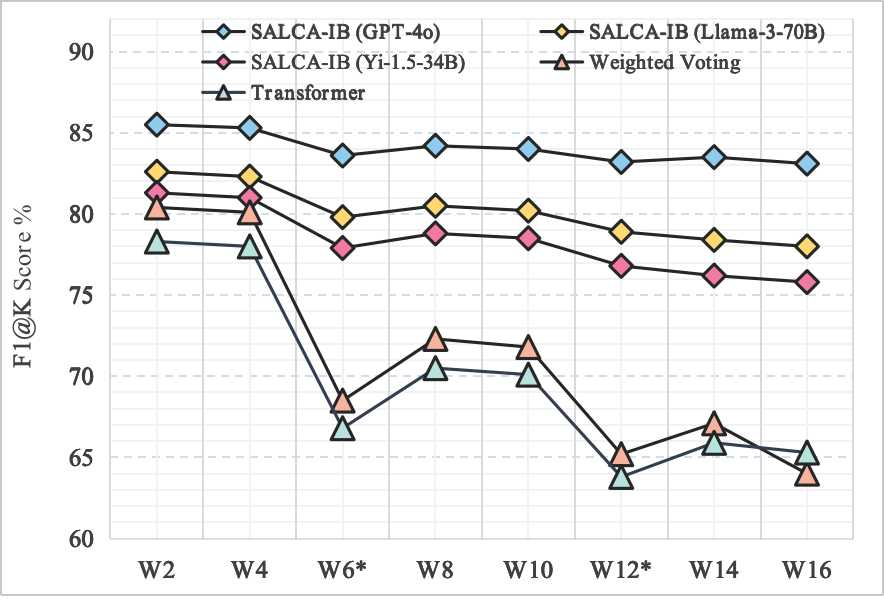
\includegraphics[width=0.45\textwidth]{fig/longtime.jpg}
    \caption{Long-term performance analysis of SALCA-IB. Week 6 and Week 12 are the two maintenance events.}
    \label{fig:salca-ib}
\end{figure}

% 随着时间变化,模型性能变化
\subsection{Long-term Performance Analysis}

To evaluate the system's robustness in real-world scenarios, we conducted a 16-week longitudinal study during which two major equipment maintenance events occurred (Week 6 and Week 12). As shown in Table \ref{tab:long_term_performance}, these maintenance activities significantly impacted the feature distributions and revealed striking differences in how various methods handled such environmental changes. During the first maintenance (Week 6), traditional methods experienced severe performance degradation, with Weighted Voting dropping by 11.6\% (80.1\% to 68.5\%) and Transformer declining by 11.2\% (78.0\% to 66.8\%). In contrast, SALCA-IB (GPT-4o) demonstrated remarkable resilience, showing only a 3.1\% decrease (85.3\% to 82.4\%). This substantial difference in impact highlights the effectiveness of our LLM-driven planning core in adapting to feature distribution shifts.

Even more revealing is the comparison between the first and second maintenance events. During the second maintenance (Week 12), SALCA-IB (GPT-4o) showed further improved resilience with only a 1.1\% performance drop (82.9\% to 81.8\%), significantly smaller than its first-event impact. This enhanced adaptability can be attributed to our dual-memory system, which effectively retained and leveraged the experience from the first maintenance event. The scale of LLM cores also played a crucial role in system resilience, as evidenced by the performance variations across different models - GPT-4o's drops (3.1\% and 1.1\%) were notably smaller than those of Llama-3-70B (4.2\% and 2.4\%) and Yi-1.5-34B (4.8\% and 2.9\%). These results collectively demonstrate SALCA-IB's robust performance in dynamic production environments, particularly through its effective combination of LLM-driven planning and experience-based adaptation.

\section{Conclusion}

This paper presents SALCA-IB, an innovative self-adaptive system for InfiniBand network failure prediction that uniquely leverages large language models as planning cores rather than direct predictors. Through extensive experiments on a production cluster with 2,048 computing cards, we demonstrate that SALCA-IB significantly outperforms traditional approaches, achieving an F1@K-score of 85.5\% in static scenarios while maintaining robust performance (83.1\%) under dynamic network conditions. The system's effectiveness is particularly evident during maintenance events, where it exhibits minimal performance degradation (3.1\% and 1.1\%) compared to traditional methods ($>$10\%). Our work advances the field through three key contributions: demonstrating LLMs' effectiveness as high-level planning cores for complex system optimization, implementing a practical dual-memory solution for knowledge accumulation in dynamic environments, and developing a continuous learning mechanism that enables sustained adaptation while maintaining prediction accuracy.

Several promising research directions emerge from this work. First, investigating lightweight LLMs could reduce computational overhead while preserving performance. Second, exploring knowledge transfer mechanisms between multiple LLM agents could enhance cross-environment learning through collaborative reasoning. Third, extending the framework to support more sophisticated LLM-driven reasoning patterns and improving system interpretability through detailed reasoning traces could increase practical utility. These directions, coupled with SALCA-IB's demonstrated success, suggest a promising path toward more robust and adaptive LLM-based infrastructure management systems capable of supporting the growing demands of large-scale AI training operations.

%\section{Ease of Use}
%
%\subsection{Maintaining the Integrity of the Specifications}
%
%The IEEEtran class file is used to format your paper and style the text. All margins, 
%column widths, line spaces, and text fonts are prescribed; please do not 
%alter them. You may note peculiarities. For example, the head margin
%measures proportionately more than is customary. This measurement 
%and others are deliberate, using specifications that anticipate your paper 
%as one part of the entire proceedings, and not as an independent document. 
%Please do not revise any of the current designations.
%
%\section{Prepare Your Paper Before Styling}
%Before you begin to format your paper, first write and save the content as a 
%separate text file. Complete all content and organizational editing before 
%formatting. Please note sections \ref{AA}--\ref{SCM} below for more information on 
%proofreading, spelling and grammar.
%
%Keep your text and graphic files separate until after the text has been 
%formatted and styled. Do not number text heads---{\LaTeX} will do that 
%for you.

%\subsection{Abbreviations and Acronyms}\label{AA}
%Define abbreviations and acronyms the first time they are used in the text, 
%even after they have been defined in the abstract. Abbreviations such as 
%IEEE, SI, MKS, CGS, ac, dc, and rms do not have to be defined. Do not use 
%abbreviations in the title or heads unless they are unavoidable.
%
%\subsection{Units}
%\begin{itemize}
%\item Use either SI (MKS) or CGS as primary units. (SI units are encouraged.) English units may be used as secondary units (in parentheses). An exception would be the use of English units as identifiers in trade, such as ``3.5-inch disk drive''.
%\item Avoid combining SI and CGS units, such as current in amperes and magnetic field in oersteds. This often leads to confusion because equations do not balance dimensionally. If you must use mixed units, clearly state the units for each quantity that you use in an equation.
%\item Do not label axes only with units. In the example, write ``Magnetization (A/m)'' or ``Magnetization \{A[m(1)]\}'', not just ``A/m''. Do not label axes with a ratio of 
%quantities and units. For example, write ``Temperature (K)'', not 
%``Temperature/K''.
%\item Use a zero before decimal points: ``0.25'', not ``.25''. Use ``cm\textsuperscript{3}'', not ``cc)''.
%\end{itemize}
%
%\subsection{Equations}
%Number equations consecutively. To make your 
%equations more compact, you may use the solidus (~/~), the exp function, or 
%appropriate exponents. Italicize Roman symbols for quantities and variables, 
%but not Greek symbols. Use a long dash rather than a hyphen for a minus 
%sign. Punctuate equations with commas or periods when they are part of a 
%sentence, as in:
%\begin{equation}
%a+b=\gamma\label{eq}
%\end{equation}
%
%Be sure that the 
%symbols in your equation have been defined before or immediately following 
%the equation. Use ``\eqref{eq}'', not ``Eq.~\eqref{eq}'' or ``equation \eqref{eq}'', except at 
%the beginning of a sentence: ``Equation \eqref{eq} is . . .''
%
%\subsection{\LaTeX-Specific Advice}
%
%Please use ``soft'' (e.g., \verb|\eqref{Eq}|) cross references instead
%of ``hard'' references (e.g., \verb|(1)|). That will make it possible
%to combine sections, add equations, or change the order of figures or
%citations without having to go through the file line by line.
%
%Please don't use the \verb|{eqnarray}| equation environment. Use
%\verb|{align}| or \verb|{IEEEeqnarray}| instead. The \verb|{eqnarray}|
%environment leaves unsightly spaces around relation symbols.
%
%Please note that the \verb|{subequations}| environment in {\LaTeX}
%will increment the main equation counter even when there are no
%equation numbers displayed. If you forget that, you might write an
%article in which the equation numbers skip from (17) to (20), causing
%the copy editors to wonder if you've discovered a new method of
%counting.
%
%{\BibTeX} does not work by magic. It doesn't get the bibliographic
%data from thin air but from .bib files. If you use {\BibTeX} to produce a
%bibliography you must send the .bib files. 
%
%{\LaTeX} can't read your mind. If you assign the same label to a
%subsubsection and a table, you might find that Table I has been cross
%referenced as Table IV-B3. 
%
%{\LaTeX} does not have precognitive abilities. If you put a
%\verb|\label| command before the command that updates the counter it's
%supposed to be using, the label will pick up the last counter to be
%cross referenced instead. In particular, a \verb|\label| command
%should not go before the caption of a figure or a table.
%
%Do not use \verb|\nonumber| inside the \verb|{array}| environment. It
%will not stop equation numbers inside \verb|{array}| (there won't be
%any anyway) and it might stop a wanted equation number in the
%surrounding equation.

%\subsection{Some Common Mistakes}\label{SCM}
%\begin{itemize}
%\item The word ``data'' is plural, not singular.
%\item The subscript for the permeability of vacuum $\mu_{0}$, and other common scientific constants, is zero with subscript formatting, not a lowercase letter ``o''.
%\item In American English, commas, semicolons, periods, question and exclamation marks are located within quotation marks only when a complete thought or name is cited, such as a title or full quotation. When quotation marks are used, instead of a bold or italic typeface, to highlight a word or phrase, punctuation should appear outside of the quotation marks. A parenthetical phrase or statement at the end of a sentence is punctuated outside of the closing parenthesis (like this). (A parenthetical sentence is punctuated within the parentheses.)
%\item A graph within a graph is an ``inset'', not an ``insert''. The word alternatively is preferred to the word ``alternately'' (unless you really mean something that alternates).
%\item Do not use the word ``essentially'' to mean ``approximately'' or ``effectively''.
%\item In your paper title, if the words ``that uses'' can accurately replace the word ``using'', capitalize the ``u''; if not, keep using lower-cased.
%\item Be aware of the different meanings of the homophones ``affect'' and ``effect'', ``complement'' and ``compliment'', ``discreet'' and ``discrete'', ``principal'' and ``principle''.
%\item Do not confuse ``imply'' and ``infer''.
%\item The prefix ``non'' is not a word; it should be joined to the word it modifies, usually without a hyphen.
%\item There is no period after the ``et'' in the Latin abbreviation ``et al.''.
%\item The abbreviation ``i.e.'' means ``that is'', and the abbreviation ``e.g.'' means ``for example''.
%\end{itemize}
%An excellent style manual for science writers is \cite{b7}.

%\subsection{Authors and Affiliations}
%\textbf{The class file is designed for, but not limited to, six authors.} A 
%minimum of one author is required for all conference articles. Author names 
%should be listed starting from left to right and then moving down to the 
%next line. This is the author sequence that will be used in future citations 
%and by indexing services. Names should not be listed in columns nor group by 
%affiliation. Please keep your affiliations as succinct as possible (for 
%example, do not differentiate among departments of the same organization).
%
%\subsection{Identify the Headings}
%Headings, or heads, are organizational devices that guide the reader through 
%your paper. There are two types: component heads and text heads.
%
%Component heads identify the different components of your paper and are not 
%topically subordinate to each other. Examples include Acknowledgments and 
%References and, for these, the correct style to use is ``Heading 5''. Use 
%``figure caption'' for your Figure captions, and ``table head'' for your 
%table title. Run-in heads, such as ``Abstract'', will require you to apply a 
%style (in this case, italic) in addition to the style provided by the drop 
%down menu to differentiate the head from the text.
%
%Text heads organize the topics on a relational, hierarchical basis. For 
%example, the paper title is the primary text head because all subsequent 
%material relates and elaborates on this one topic. If there are two or more 
%sub-topics, the next level head (uppercase Roman numerals) should be used 
%and, conversely, if there are not at least two sub-topics, then no subheads 
%should be introduced.

%\subsection{Figures and Tables}
%\paragraph{Positioning Figures and Tables} Place figures and tables at the top and 
%bottom of columns. Avoid placing them in the middle of columns. Large 
%figures and tables may span across both columns. Figure captions should be 
%below the figures; table heads should appear above the tables. Insert 
%figures and tables after they are cited in the text. Use the abbreviation 
%``Fig.~\ref{fig}'', even at the beginning of a sentence.
%
%\begin{table}[htbp]
%\caption{Table Type Styles}
%\begin{center}
%\begin{tabular}{|c|c|c|c|}
%\hline
%\textbf{Table}&\multicolumn{3}{|c|}{\textbf{Table Column Head}} \\
%\cline{2-4} 
%\textbf{Head} & \textbf{\textit{Table column subhead}}& \textbf{\textit{Subhead}}& \textbf{\textit{Subhead}} \\
%\hline
%copy& More table copy$^{\mathrm{a}}$& &  \\
%\hline
%\multicolumn{4}{l}{$^{\mathrm{a}}$Sample of a Table footnote.}
%\end{tabular}
%\label{tab1}
%\end{center}
%\end{table}
%
%
%Figure Labels: Use 8 point Times New Roman for Figure labels. Use words 
%rather than symbols or abbreviations when writing Figure axis labels to 
%avoid confusing the reader. As an example, write the quantity 
%``Magnetization'', or ``Magnetization, M'', not just ``M''. If including 
%units in the label, present them within parentheses. Do not label axes only 
%with units. In the example, write ``Magnetization (A/m)'' or ``Magnetization 
%\{A[m(1)]\}'', not just ``A/m''. Do not label axes with a ratio of 
%quantities and units. For example, write ``Temperature (K)'', not 
%``Temperature/K''.

%\section*{Acknowledgment}
%
%The preferred spelling of the word ``acknowledgment'' in America is without 
%an ``e'' after the ``g''. Avoid the stilted expression ``one of us (R. B. 
%G.) thanks $\ldots$''. Instead, try ``R. B. G. thanks$\ldots$''. Put sponsor 
%acknowledgments in the unnumbered footnote on the first page.

%\section*{References}
%
%Please number citations consecutively within brackets \cite{b1}. The 
%sentence punctuation follows the bracket \cite{b2}. Refer simply to the reference 
%number, as in \cite{b3}---do not use ``Ref. \cite{b3}'' or ``reference \cite{b3}'' except at 
%the beginning of a sentence: ``Reference \cite{b3} was the first $\ldots$''
%
%Number footnotes separately in superscripts. Place the actual footnote at 
%the bottom of the column in which it was cited. Do not put footnotes in the 
%abstract or reference list. Use letters for table footnotes.
%
%Unless there are six authors or more give all authors' names; do not use 
%``et al.''. Papers that have not been published, even if they have been 
%submitted for publication, should be cited as ``unpublished'' \cite{b4}. Papers 
%that have been accepted for publication should be cited as ``in press'' \cite{b5}. 
%Capitalize only the first word in a paper title, except for proper nouns and 
%element symbols.
%
%For papers published in translation journals, please give the English 
%citation first, followed by the original foreign-language citation \cite{b6}.

\newpage
\begin{thebibliography}{00}
\bibitem{b1} T. Ahmed, S. Ghosh, C. Bansal, T. Zimmermann, X. Zhang, S. Rajmohan et al., "Recommending root-cause and mitigation steps for cloud incidents using large language models," in Proc. IEEE/ACM 45th Int. Conf. Software Engineering (ICSE), Melbourne, Australia, 2023, pp. 1737-1749.

\bibitem{b2} K. A. Alharthi, A. Jhumka, S. Di, L. Gui, F. Cappello, S. McIntosh-Smith, "Time machine: Generative real-time model for failure (and lead time) prediction in HPC systems," in Proc. 53rd Annual IEEE/IFIP Int. Conf. Dependable Systems and Networks (DSN), 2023, pp. 508-521.

\bibitem{b3} F. Antici, A. Borghesi, and Z. Kiziltan, "Online job failure prediction in an HPC system," in Euro-Par 2023: Parallel Processing Workshops, Cham: Springer, 2024, pp. 167-179.

\bibitem{b4} A. Cascajo, G. Gomez-Lopez, J. Escudero-Sahuquillo, P. J. Garcia, D. E. Singh, F. Alfaro-Cortés et al., "Monitoring infiniband networks to react efficiently to congestion," IEEE Micro, vol. 43, no. 2, pp. 120-130, 2023.

\bibitem{b5} A. Das, F. Mueller, C. Siegel, and A. Vishnu, "Desh: Deep learning for system health prediction of lead times to failure in HPC," in Proc. 27th Int. Symp. High-Performance Parallel and Distributed Computing, 2018, pp. 40-51.

\bibitem{b6} Y. He, M. Hutton, S. Chan, R. De Gruijl, R. Govindaraju, N. Patil et al., "Understanding and mitigating hardware failures in deep learning training systems," in Proc. 50th Annual Int. Symp. Computer Architecture, 2023, pp. 1-16.

\bibitem{b7} Q. Hu, Z. Ye, Z. Wang, G. Wang, M. Zhang, Q. Chen et al., "Characterization of large language model development in the datacenter," in Proc. USENIX Symp. Networked Systems Design and Implementation (NSDI), 2024, pp. 709-729.

\bibitem{b8} H. Liu, Z. Li, C. Tan, R. Yang, G. Cao, Z. Liu et al., "Predicting GPU failures with high precision under deep learning workloads," in Proc. 16th ACM Int. Conf. Systems and Storage, 2023, pp. 124-135.

\bibitem{b9} B. Mohammed, I. Awan, H. Ugail, and M. Younas, "Failure prediction using machine learning in a virtualised HPC system and application," Cluster Computing, vol. 22, no. 2, pp. 471-485, 2019.

\bibitem{b10} B. Nie, J. Xue, S. Gupta, T. Patel, C. Engelmann, E. Smirni et al., "Machine learning models for GPU error prediction in a large scale HPC system," in Proc. 48th Annual IEEE/IFIP Int. Conf. Dependable Systems and Networks (DSN), 2018, pp. 95-106.

\bibitem{b11} R. Rajachandrasekar, X. Besseron, and D. K. Panda, "Monitoring and predicting hardware failures in HPC clusters with FTB-IPMI," in Proc. IEEE 26th Int. Parallel and Distributed Processing Symp. Workshops \& PhD Forum, 2012, pp. 1136-1143.

\bibitem{b12} J. Su, C. Jiang, X. Jin, Y. Qiao, T. Xiao, H. Ma et al., "Large language models for forecasting and anomaly detection: A systematic literature review," arXiv preprint arXiv:2402.10350, 2024.

\bibitem{b13} T. Zhang, X. Huang, W. Zhao, S. Bian, and P. Du, "LogPrompt: A log-based anomaly detection framework using prompts," in Proc. Int. Joint Conf. Neural Networks (IJCNN), 2023, pp. 1-8.

\bibitem{madaan2023} A. Madaan, N. Tandon, P. Gupta, S. Hallinan, L. Gao, S. Wiegreffe et al., "Self-Refine: Iterative refinement with self-feedback," in Advances in Neural Information Processing Systems, vol. 36, 2023, pp. 46534-46594.

\bibitem{weng2023} Y. Weng, M. Zhu, F. Xia, B. Li, S. He, S. Liu, B. Sun, K. Liu, J. Zhao, "Large Language Models are Better Reasoners with Self-Verification," in Findings of EMNLP 2023.

\bibitem{tyen2023} G. Gladys Tyen, Hassan Mansoor, Victor Cărbune, Peter Chen, Tony Mak, "LLMs cannot find reasoning errors, but can correct them given the error location," in Findings of ACL 2024.

\bibitem{shridhar2023} Kumar Shridhar, Koustuv Sinha, Andrew Cohen, Tianlu Wang, Ping Yu, Ram Pasunuru, Mrinmaya Sachan, Jason Weston, Asli Celikyilmaz, "The ART of LLM Refinement: Ask, Refine, and Trust," arXiv preprint arXiv:2311.07961, 2023.

\bibitem{chen2023} X. Chen, S. Zhang, Y. Zhang, H. Zhang, P. Zhao, and Q. Jin, "Chain-of-Thought Prompting Elicits Reasoning in Large Language Models," in Proc. NeurIPS 2023.

\bibitem{wang2023} Xuezhi Wang, Jason Wei, Dale Schuurmans, Quoc Le, Ed Chi, Sharan Narang, Aakanksha Chowdhery, Denny Zhou, "Self-Consistency Improves Chain of Thought Reasoning in Language Models," in Proc. ICLR 2023.

\bibitem{krishnamurthy2023} R. Krishnamurthy, A. Kumar, S. Basu, S. Maji, V. Balasubramanian, and P. Liang, "HierarchicalMem: An Adaptive Memory System for Large Language Models," in Proc. EMNLP 2023.

\bibitem{li2023} J. Li, Z. Yang, X. Jiang, Y. Luo, S. Zhang, and J. Yang, "Efficient Memory Management for Large Language Model Serving with PagedAttention," in Proc. SOSP 2023.

\bibitem{liu2023} H. Liu, K. Wang, Q. Chen, Z. Yang, J. Deng, and D. Wang, "Iterative Refinement of Large Language Model Outputs with Feedback Loops," in Proc. ACL 2023.

\bibitem{zhao2023} Z. Zhao, R. Liu, K. Chen, D. Wei, W. Shi, and D. Song, "Meta-Learning for Adaptive Large Language Models," in Proc. ICML 2023.

\bibitem{an2024} S. An, Z. Ma, Z. Lin, N. Zheng, J.-G. Lou, and W. Chen, "Learning from mistakes makes LLM better reasoner," arXiv preprint arXiv:2310.20689, 2024.

\bibitem{gao2024} J. Gao, X. Ding, Y. Cui, J. Zhao, H. Wang, T. Liu, and B. Qin, "Self-evolving GPT: A lifelong autonomous experiential learner," arXiv preprint arXiv:2407.08937, 2024.

\bibitem{gou2024} Z. Gou, Z. Shao, Y. Gong, Y. Shen, Y. Yang, N. Duan, and W. Chen, "CRITIC: Large language models can self-correct with tool-interactive critiquing," arXiv preprint arXiv:2305.11738, 2024.

\bibitem{qiao2024} S. Qiao, H. Gui, C. Lv, Q. Jia, H. Chen, and N. Zhang, "Making language models better tool learners with execution feedback," arXiv preprint arXiv:2305.13068, 2024.

\bibitem{shinn2023} N. Shinn, F. Cassano, E. Berman, A. Gopinath, K. Narasimhan, and S. Yao, "Reflexion: Language agents with verbal reinforcement learning," arXiv preprint arXiv:2303.11366, 2023.

\bibitem{wang2024} J. Wang, J. Wang, B. Athiwaratkun, C. Zhang, and J. Zou, "Mixture-of-agents enhances large language model capabilities," arXiv preprint arXiv:2406.04692, 2024.

\bibitem{wang2024agent} Z. Z. Wang, J. Mao, D. Fried, and G. Neubig, "Agent workflow memory," arXiv preprint arXiv:2409.07429, 2024.

\bibitem{yao2023} Shunyu Yao, Jeffrey Zhao, Dian Yu, Nan Du, Izhak Shafran, Karthik Narasimhan, Yuan Cao, "ReAct: Synergizing reasoning and acting in language models," arXiv preprint arXiv:2210.03629, 2023.

\bibitem{cao2024} D. Cao, F. Jia, S. O. Arik, T. Pfister, Y. Zheng, W. Ye, and Y. Liu, "TEMPO: Prompt-based generative pre-trained transformer for time series forecasting," arXiv preprint arXiv:2310.04948, 2024.

\bibitem{chang2024} C. Chang, W.-Y. Wang, W.-C. Peng, and T.-F. Chen, "LLM4TS: Aligning pre-trained LLMs as data-efficient time-series forecasters," arXiv preprint arXiv:2308.08469, 2024.

\bibitem{gruver2023} N. Gruver, M. Finzi, S. Qiu, and A. G. Wilson, "Large language models are zero-shot time series forecasters," in Advances in Neural Information Processing Systems, vol. 36, 2023, pp. 19622-19635.

\bibitem{jin2024} M. Jin, S. Wang, L. Ma, Z. Chu, J. Y. Zhang, X. Shi, P. Y. Chen, Y. Liang, Y. F. Li, S. Pan, Q. Wen, "Time-LLM: Time series forecasting by reprogramming large language models," arXiv preprint arXiv:2310.01728, 2024.

\bibitem{xue2023} H. Xue and F. D. Salim, "PromptCast: A new prompt-based learning paradigm for time series forecasting," arXiv preprint arXiv:2210.08964, 2023.

\bibitem{zhou2023} T. Zhou, P. Niu, X. Wang, L. Sun, and R. Jin, "One fits all: Power general time series analysis by pretrained LM," in Advances in Neural Information Processing Systems, vol. 36, 2023, pp. 43322-43355.
\end{thebibliography}
\vspace{12pt}
%\color{red}
%IEEE conference templates contain guidance text for composing and formatting conference papers. Please ensure that all template text is removed from your conference paper prior to submission to the conference. Failure to remove the template text from your paper may result in your paper not being published.

\section{Appendix}

\subsection{The SALCA-IB Algorithm}
\begin{algorithm}[H]
    \caption{Self-Adaptive Learning with Continuous Assessment (SALCA-IB)}
    \label{alg:salca-ib}
    \begin{algorithmic}[1]
    \Require
        \Statex \hspace{-1em}Network monitoring data $\mathcal{D} = \{(X_t, y_t)\}_{t=1}^T$
        \Statex \hspace{-1em}Large language model $\mathcal{L}$ with prompt templates $\mathcal{P}$
        \Statex \hspace{-1em}Model pool $\mathcal{M} = \{M_1, ..., M_m\}$
        \Statex \hspace{-1em}Dual-memory system: $Mem_{short} = \{F_{current}, T_{range}, P_{model}, M_{config}, F_{recent}\}$
        \Statex \hspace{-1em}\hspace{3.6em}$Mem_{long} = \{F_{stats}, M_{history}, E_{record}, A_{track}, F_{history}\}$
    
    \Ensure Optimized ensemble model $M_{ensemble}$, Updated memory system
    
    \vspace{0.5em}
    \Function{InitializeSystem}{$\mathcal{D}, \mathcal{M}, Mem_{long}$}
        \State $D_{train} \gets LLM(\mathcal{D}, Mem_{long}, \mathcal{P}_{select})$  \\
        \Comment{Knowledge-driven data selection}
        \State $(M_{selected}, \Theta, S) \gets LLM(\mathcal{M}, Mem_{long}, \mathcal{P}_{config})$  \\
        \Comment{Model configuration and ensemble strategy}
        \State $M_{ensemble} \gets TrainEnsemble(M_{selected}, \Theta, S, D_{train})$
        \State \Return $M_{ensemble}, D_{train}$
    \EndFunction
    
    \Function{ContinuousLearning}{$M_{ensemble}, \mathcal{D}_{new}$}
        \While{$\text{not converged}$}
            \State $P_t \gets Predict(M_{ensemble}, X_t)$  \\
            \Comment{Generate failure predictions}
            \State $E_t \gets Evaluate(P_t, y_t)$  \\
            \Comment{Assess prediction performance}
            
            \State // Feedback generation and analysis
            \State $f_t \gets LLM(E_t, Mem_{long}, \mathcal{P}_{analyze})$  \\
            \Comment{Generate structured feedback}
            \State $I_t \gets LLM(f_t, F_{history}, \mathcal{P}_{improve})$  \\
            \Comment{Develop improvement strategies}
            \State $V_t \gets LLM(I_t, F_{history}, \mathcal{P}_{validate})$  \\
            \Comment{Validate proposed strategies}
            
            \State // Memory system operations
            \State $UpdateMemory(Mem_{short}, f_t, E_t, P_t)$  \\
            \Comment{Update short-term memory}
            \State $TransferMemory(Mem_{short}, Mem_{long})$ \\
            \Comment{Transfer valuable experiences}
            \State $CleanupMemory(A_{track}, \tau_{active})$ \\
            \Comment{Remove inactive entries}
            
            \State // System optimization
            \State $C_{t+1} \gets Optimize(C_t, V_t, \mathcal{P}_{refine})$ \\
            \Comment{Apply validated improvements}
            \State $M_{ensemble}.update(C_{t+1}, \mathcal{D}_{new})$ \\
            \Comment{Update ensemble model}
            
            \State // Activation tracking
            \State $A_{track} \gets UpdateActivation(A_{track}, f_t)$ \\
            \Comment{Update memory activation status}
        \EndWhile
        \State \Return $M_{ensemble}, Mem_{short}, Mem_{long}$
    \EndFunction
    
    \State Main process
    \State $M_{ensemble}, D_{train} \gets \text{InitializeSystem}(\mathcal{D}, \mathcal{M}, Mem_{long})$
    \State $M_{ensemble}, Mem_{short}, Mem_{long} \gets \text{ContinuousLearning}(M_{ensemble}, \mathcal{D}_{new})$ 
    \State \Return $M_{ensemble}, Mem_{short}, Mem_{long}$
    \end{algorithmic}
\end{algorithm}

\begin{table}[!t]
\caption{Model Pool Configuration Options with LLM Selection Examples}
\label{tab:model_config}
\begin{center}
\begin{tabular}{|p{2.5cm}|p{5cm}|}
\hline
\multicolumn{2}{|c|}{\textbf{Model Architecture Parameters}} \\
\hline
\textbf{Model Type} & \textbf{Parameter Range (Example Choice)} \\
\hline
\multirow{4}{*}{MLP} & Layers: [3-6] (4) \\
& Units: [64,128,256,512] (128) \\
& Dropout: [0.1-0.5] (0.3) \\
& Width decay ratio: [1.5-3.0] (2.0) \\
\hline
\multirow{4}{*}{CNN} & Conv layers: [1-5] (3) \\
& Filters: [32,64,128] (64) \\
& Kernel size: [3,5,7] (3) \\
& Pooling: [Max, Average] (Max) \\
\hline
\multirow{4}{*}{LSTM} & Layers: [1-8] (4) \\
& Hidden units: [64,128,256,512] (128) \\
& Dropout: [0.1-0.5] (0.4) \\
& Sequence length: [10-50] (30) \\
\hline
\multirow{4}{*}{GRU} & Layers: [1-4] (3) \\
& Hidden units: [64,128,256,512] (256) \\
& Dropout: [0.1-0.5] (0.3) \\
& Update gate bias: [-2.0,2.0] (1.0) \\
\hline
\multirow{4}{*}{Transformer} & Layers: [2-8] (6) \\
& Embedding dim: [128,256,512] (256) \\
& Dropout: [0.1-0.5] (0.5) \\
& Attention heads: [4,8,16] (8) \\
\hline
\multicolumn{2}{|c|}{\textbf{Training Parameters}} \\
\hline
\multicolumn{2}{|l|}{Batch size: [32-512] (64)} \\
\multicolumn{2}{|l|}{Learning rate: [1e-5, 1e-4, 1e-3] (5e-4)} \\
\multicolumn{2}{|l|}{Optimizer: AdamW with weight decay [1e-5, 1e-3] (1e-4)} \\
\multicolumn{2}{|l|}{Early stopping patience: [5-20 epochs] (10)} \\
\hline
\end{tabular}
\end{center}
\end{table}

\begin{table}[!t]
\caption{Appendix: InfiniBand Card Monitoring Metrics}
\label{tab:appendix_metrics}
\renewcommand{\arraystretch}{1.2}
\begin{center}
\begin{tabular}{l|l|l}
\hline
\textbf{Category} & \textbf{Metric Name} & \textbf{Value Range} \\
\hline
\multirow{11}{*}{\makecell[l]{Performance \& \\ Error Diagnostics\\(36 metrics)}} 
& Link State & {Active, Down} \\
& Physical State & {LinkUp, LinkDown} \\
& DataPath State (×4) & {DPActivated, DPDeactivated} \\
& CDR Status (×4) & {ON, OFF} \\
& Tx/Rx CDR LOL (×4) & Binary \\
& Tx/Rx LOS (×4) & Binary \\
& Tx/Rx Fault (×4) & Binary \\
& FW Fault & Binary \\
& Error Code Response & {ConfigUndefined, ...} \\
& Eye Opening Score & [0, 100] \\
& ... & ... \\
\hline
\multirow{2}{*}{\makecell[l]{Temperature\\(2 metrics)}} 
& Module Temperature & [-10, 80]°C \\
& Case Temperature & [-10, 85]°C \\
\hline
\multirow{8}{*}{\makecell[l]{Physical\\Parameters\\(17 metrics)}} 
& Module Voltage & [2970, 3630]mV \\
& Bias Current (×4) & [0, 15]mA \\
& Rx Power (×4) & [-10.41, 5]dBm \\
& Tx Power (×4) & [-8.416, 5]dBm \\
& Link Speed & {SDR...NDR} \\
& Link Width & {1x, 2x, 4x} \\
& Wavelength & [840, 860]nm \\
& Power Class & [0, 8.0]W \\
\hline
\end{tabular}
\end{center}
\end{table}

\end{document}
